\documentclass[a4paper,10pt]{article}

\usepackage[english]{babel}
\usepackage{graphicx}
\usepackage{amsmath}

\usepackage{float} % for [H]
\usepackage[colorlinks, linkcolor=black, citecolor=black, urlcolor=black]{hyperref}
\usepackage{geometry}
\geometry{tmargin=3cm, bmargin=2.2cm, lmargin=2.2cm, rmargin=2cm}
\usepackage{todonotes} %Used for the figure placeholders
\usepackage{ifthen}
\usepackage{booktabs} %For better table formatting
\usepackage{longtable} %For tables that span multiple pages
\usepackage{array} %For column formatting
\usepackage{tabularx} %For flexible table column widths
\usepackage{tikz}
\usetikzlibrary{shapes, arrows.meta, positioning, fit, backgrounds, calc}
\usepackage{listings}
\usepackage{xcolor}

% Modern light code listing style for C
\definecolor{codebg}{RGB}{250,250,250}
\definecolor{codecomment}{RGB}{106,115,125}
\definecolor{codestring}{RGB}{80,161,79}
\definecolor{codekeyword}{RGB}{167,29,93}
\definecolor{codenumber}{RGB}{150,150,150}
\definecolor{codetext}{RGB}{36,41,46}
\definecolor{codeborder}{RGB}{225,228,232}

\lstdefinestyle{cstyle}{
    backgroundcolor=\color{codebg},
    commentstyle=\color{codecomment}\itshape,
    keywordstyle=\color{codekeyword},
    numberstyle=\tiny\color{codenumber},
    stringstyle=\color{codestring},
    basicstyle=\ttfamily\scriptsize\color{codetext},
    breakatwhitespace=false,
    breaklines=true,
    captionpos=b,
    keepspaces=true,
    numbers=left,
    numbersep=8pt,
    showspaces=false,
    showstringspaces=false,
    showtabs=false,
    tabsize=4,
    frame=single,
    framerule=0.5pt,
    rulecolor=\color{codeborder},
    xleftmargin=1.5em,
    framexleftmargin=1em,
    framextopmargin=4pt,
    framexbottommargin=4pt,
    aboveskip=1em,
    belowskip=0.5em
}

\setlength{\parindent}{0pt}

% Your name and student number must be filled in on the title page found in
% titlepage.tex.

\begin{document}
\newboolean{anonymize}
% Uncomment to create an anonymized version of your report
%\setboolean{anonymize}{true}

\begin{titlepage}
    \newpage
    \thispagestyle{empty}
    \frenchspacing
    \hspace{-0.2cm}
    \includegraphics[height=3.4cm]{sedes}
    \hspace{0.2cm}
    \rule{0.5pt}{3.4cm}
    \hspace{0.2cm}
    \begin{minipage}[b]{8cm}
        \Large{Katholieke\newline Universiteit\newline Leuven}\smallskip\newline
        \large{}\smallskip\newline
        \textbf{Master of Engineering Science\newline Artificial Intelligence}\smallskip
    \end{minipage}
    \hspace{\stretch{1}}
    \vspace*{3.2cm}\vfill
    \begin{center}
        \begin{minipage}[t]{\textwidth}
            \begin{center}
                \LARGE{\rm{\textbf{\uppercase{Privacy Impact Assessment}}}}\\
                \Large{\rm{Macless-Haystack}}
            \end{center}
        \end{minipage}
    \end{center}
    \vfill
    \hfill\makebox[8.5cm][l]{%
        \vbox to 7cm{\vfill\noindent
            \ifthenelse{\boolean{anonymize}}{%
                {\rm \textbf{Anonymized}}\\
                {\rm Academic year 2025--2026}
            }{%
                {\rm \textbf{Lili De Bruyn (r0848166)}}\\
                {\rm \textbf{Annemerel Bobbaers (r0897155)}}\\
                {\rm \textbf{Magnus De Maerteleire (r0889456)}}\\
                {\rm \textbf{Jeff Jambé (r0902205)}}\\[2mm]
                {\rm Academic year 2025--2026}
            }
        }
    }
\end{titlepage}


\tableofcontents
\newpage

% Introduction/Executive Summary
\section{Introduction}
This report presents a Privacy Impact Assessment (PIA) for Macless-Haystack \cite{maclesshaystack}, an open-source project that enables users to access Apple's Find My network without requiring Apple hardware. As location tracking systems become increasingly prevalent, understanding the privacy implications of such technologies is crucial for both developers and end users.
\bigskip

The assessment examines how Macless-Haystack collects, processes, and stores location data, identifies potential privacy risks, and proposes technical solutions to mitigate these concerns. We analyze the system from multiple perspectives: the tracker devices themselves, the Macless-Haystack application and API, and Apple's Find My infrastructure that the project relies upon.
\bigskip

This report is structured in three main parts. First, we provide a detailed description of the application's functionality, stakeholders, and data collection practices. Second, we conduct a privacy impact assessment that includes a threat model, identification of privacy issues, and analysis of specific threats. Finally, we present recommendations for addressing the identified privacy concerns, with particular focus on technical implementations that can be tested and verified.

% Part 1: Application Description (max 1500 words)
\section{Application Description}

\subsection{Functionality of the Application}
Macless-Haystack builds upon the OpenHaystack \cite{openhaystack} project, which reverse engineered the Apple 'Find My' protocol that enables tracking of Bluetooth devices without the need of an internet connection.
\bigskip

At a high level, the Find My trackers broadcast identifiers, which can be detected by nearby Apple devices. These Apple devices then anonymously upload the location of the detected signal to iCloud. The owner can later retrieve the location of their device by requesting reports containing the trackers identifier.
\bigskip

Figure~\ref{fig:macless-haystack} below visually represents the four main stages of the application:

\begin{enumerate}
    \item \textbf{Pair through initial setup}: The process begins with the owner pairing their device, this means generating a unique private-public key pair. These keys are programmed onto supported Bluetooth devices.
    \item \textbf{Broadcast}: After setup, the tracker begins broadcasting Bluetooth advertisements that are based on its public key. Apple devices nearby act as a finder device and can pick up on these advertisements.
    \item \textbf{Upload encrypted location reports}: When a finder device detects an advertisement, it generates a report containing its current GPS location. This location is then encrypted using the advertisement key broadcasted by the device, making it inaccessible to everyone except the owner. The encrypted report is uploaded to Apple's servers, with no way for Apple to decipher the actual location.
    \item \textbf{Download and decrypt location reports}: Any device authenticated with the owner's Apple ID can request location reports linked to the tracker's keys. Using the matching advertisement key, the owner can decrypt these reports and see each location on a map.
\end{enumerate}

Macless-Haystack gets rid of the need for any Apple hardware. All you need is an Apple ID with two-factor authentication via SMS and either a linux device or a supported bluetooth enabled microcontroller.

\begin{figure}[]
    \centering
    \includegraphics[width=0.8\textwidth]{figures/applicationoverview.png}
    \caption{High-level overview of the Macless-Haystack workflow}
    \label{fig:macless-haystack}
\end{figure}


\subsection{The Stakeholders}
The primary stakeholders are the end users who want to track their own Bluetooth devices via Apple's Find My network using Macless-Haystack's web browser. They provide an Apple ID, password, and SMS-based two-factor authentication once when setting up the Macless-Haystack endpoint container, and then interact with the system via a browser to import device key JSON files, view locations, filter by date, and export data. End users are responsible for generating and managing tracker keys and deciding which devices are associated with their Apple ID; they are the primary beneficiaries of the system's tracking functionality.
\bigskip

The Macless-Haystack endpoint operator is the party running the backend container that logs into Apple's Find My service and periodically fetches encrypted location reports, typically on a server with Docker installed. In many cases this is the same party as the end user.
\bigskip

The Anisette server operator runs the separate Anisette-compatible service that Macless-Haystack connects to in order to emulate a real Apple device during login and communication with Apple. This role can again coincide with the endpoint operator in a self-hosted setup, but when a public or third-party Anisette instance is used, that operator becomes a distinct stakeholder who may see sensitive authentication-related traffic and must therefore be explicitly trusted.
\bigskip

Apple is an indirect but essential stakeholder, as its Find My and iCloud infrastructure receives the encrypted location reports from nearby Apple devices and serves them to the Macless-Haystack endpoint authenticated with an Apple ID.

\subsection{Types of Data Collected and Purposes}

\subsubsection{Data Collection in the Tracker}
The tracker itself does not collect any data. It operates solely using the public key that is provided to it.

\subsubsection{Data Collection in Apple's System}
Because Apple's implementation is closed-source, we can only make informed assumptions about what data is collected. For completeness, we assume that Apple collects all data that is technically available to it.

Crowd-sourced Apple devices collect only three pieces of information when they detect a tracker:
\begin{itemize}
    \item the advertisement key,
    \item the device's location at the moment of detection,
    \item and the Bluetooth signal strength at that time.
\end{itemize}

According to a blog by a Digital Forensics researcher at cellebrite\cite{binaryhick2025searchparty}, this data is normally deleted quickly, but users can delay deletion by placing their device in airplane mode. This data is placed on the apple servers, and used for people to retrieve the location of their tracker reference.
\bigskip

Apple stores the advertisement key together with its corresponding location report on their servers. From this, Apple can infer how many trackers are in use and estimate the general region in which they are being used, based on the uploader's IP address. Apple also knows the Apple ID associated with each device that uploads these reports. This means, at least in theory, that Apple could link a user to their tracker because the user's own Apple device will likely often be the one uploading the tracker's location reports.
\bigskip

Fetching location reports requires authentication. As a result, Apple can see which Apple account is hosting a Macless-Haystack endpoint and which trackers are used through that endpoint. This could allow Apple to terminate the Apple ID associated with the endpoint. The requirement for Apple ID authentication is likely in place to prevent abuse such as users uploading spam, overwhelming Apple's servers, or attempting to download large volumes of location reports that aren't their own.

\subsubsection{Data Collected by the Macless-Haystack Application}
The Macless-Haystack frontend stores very little data. The single-page browser interface keeps the private keys of imported trackers in secure local storage. It also stores the username and password used to authenticate with the macless-haystack endpoint; however, these credentials are stored in plain text.
During the use of the application, the current and past location of all trackers is stored in cache.

\subsubsection{Data Collected by the Macless-Haystack API}
The API stores only minimal data, but it logs a significant amount of sensitive information. This includes every request made by the application, which means that if the logs are reviewed, the advertisement keys of all Macless-Haystack trackers can be seen.
\bigskip

\begin{table}[H]
    \centering
    \caption{Summary of Data Collection, Storage, and Retention}
    \label{tab:data_collection_summary}
    \begin{tabularx}{\textwidth}{|>{\raggedright\arraybackslash}X|>{\raggedright\arraybackslash}p{2cm}|>{\raggedright\arraybackslash}X|>{\raggedright\arraybackslash}p{2cm}|>{\raggedright\arraybackslash}X|}
        \hline
        \textbf{Data Item} & \textbf{Source} & \textbf{Storage Location} & \textbf{Retention Period} & \textbf{Potential Privacy Impact} \\ \hline
        Apple ID / Credentials & endpoint operator & JSON in API Backend & Indefinite & Full account compromise; access to other Apple services. \\ \hline
        Public \& Private Key(s) & End User & Browser Local Storage \& JSON in filesystem \& tracker firmware / flash storage & Indefinite & Unauthorized access to (historical) location data. \\ \hline
        Advertisement Keys & Tracker / Finder Device & Apple Servers, API Logs & Apple: $<24$h; Logs: Persistent & Linkability; device/owner movement profiling by nearby observers. \\ \hline
        Location Reports & Finder Device & Apple Servers & Short-term ($\sim$24h) & Exposure of real-time/historical physical locations and routines. \\ \hline
    \end{tabularx}
\end{table}

% Part 2: Privacy Impact Assessment (max 2500 words)
\section{Privacy Impact Assessment}

\subsection{Threat Model}
The system's privacy properties depend on several trust assumptions. Users must trust Apple's infrastructure to provide end-to-end encryption (though Apple has metadata visibility), the endpoint operator to protect stored credentials and logs, and any third-party Anisette server operator to handle authentication securely. The primary trust boundaries exist at: (1) Bluetooth broadcast between tracker and nearby devices, (2) network communication between frontend and backend (currently vulnerable when HTTP is used), (3) authenticated connections to Apple's servers (which reveal query metadata), and (4) filesystem access on the server (where plaintext credentials are stored). These boundaries represent the main points where information can be compromised, as detailed in the threat analysis below.    
\begin{figure}[ht]
    \centering
    \resizebox{\textwidth}{!}{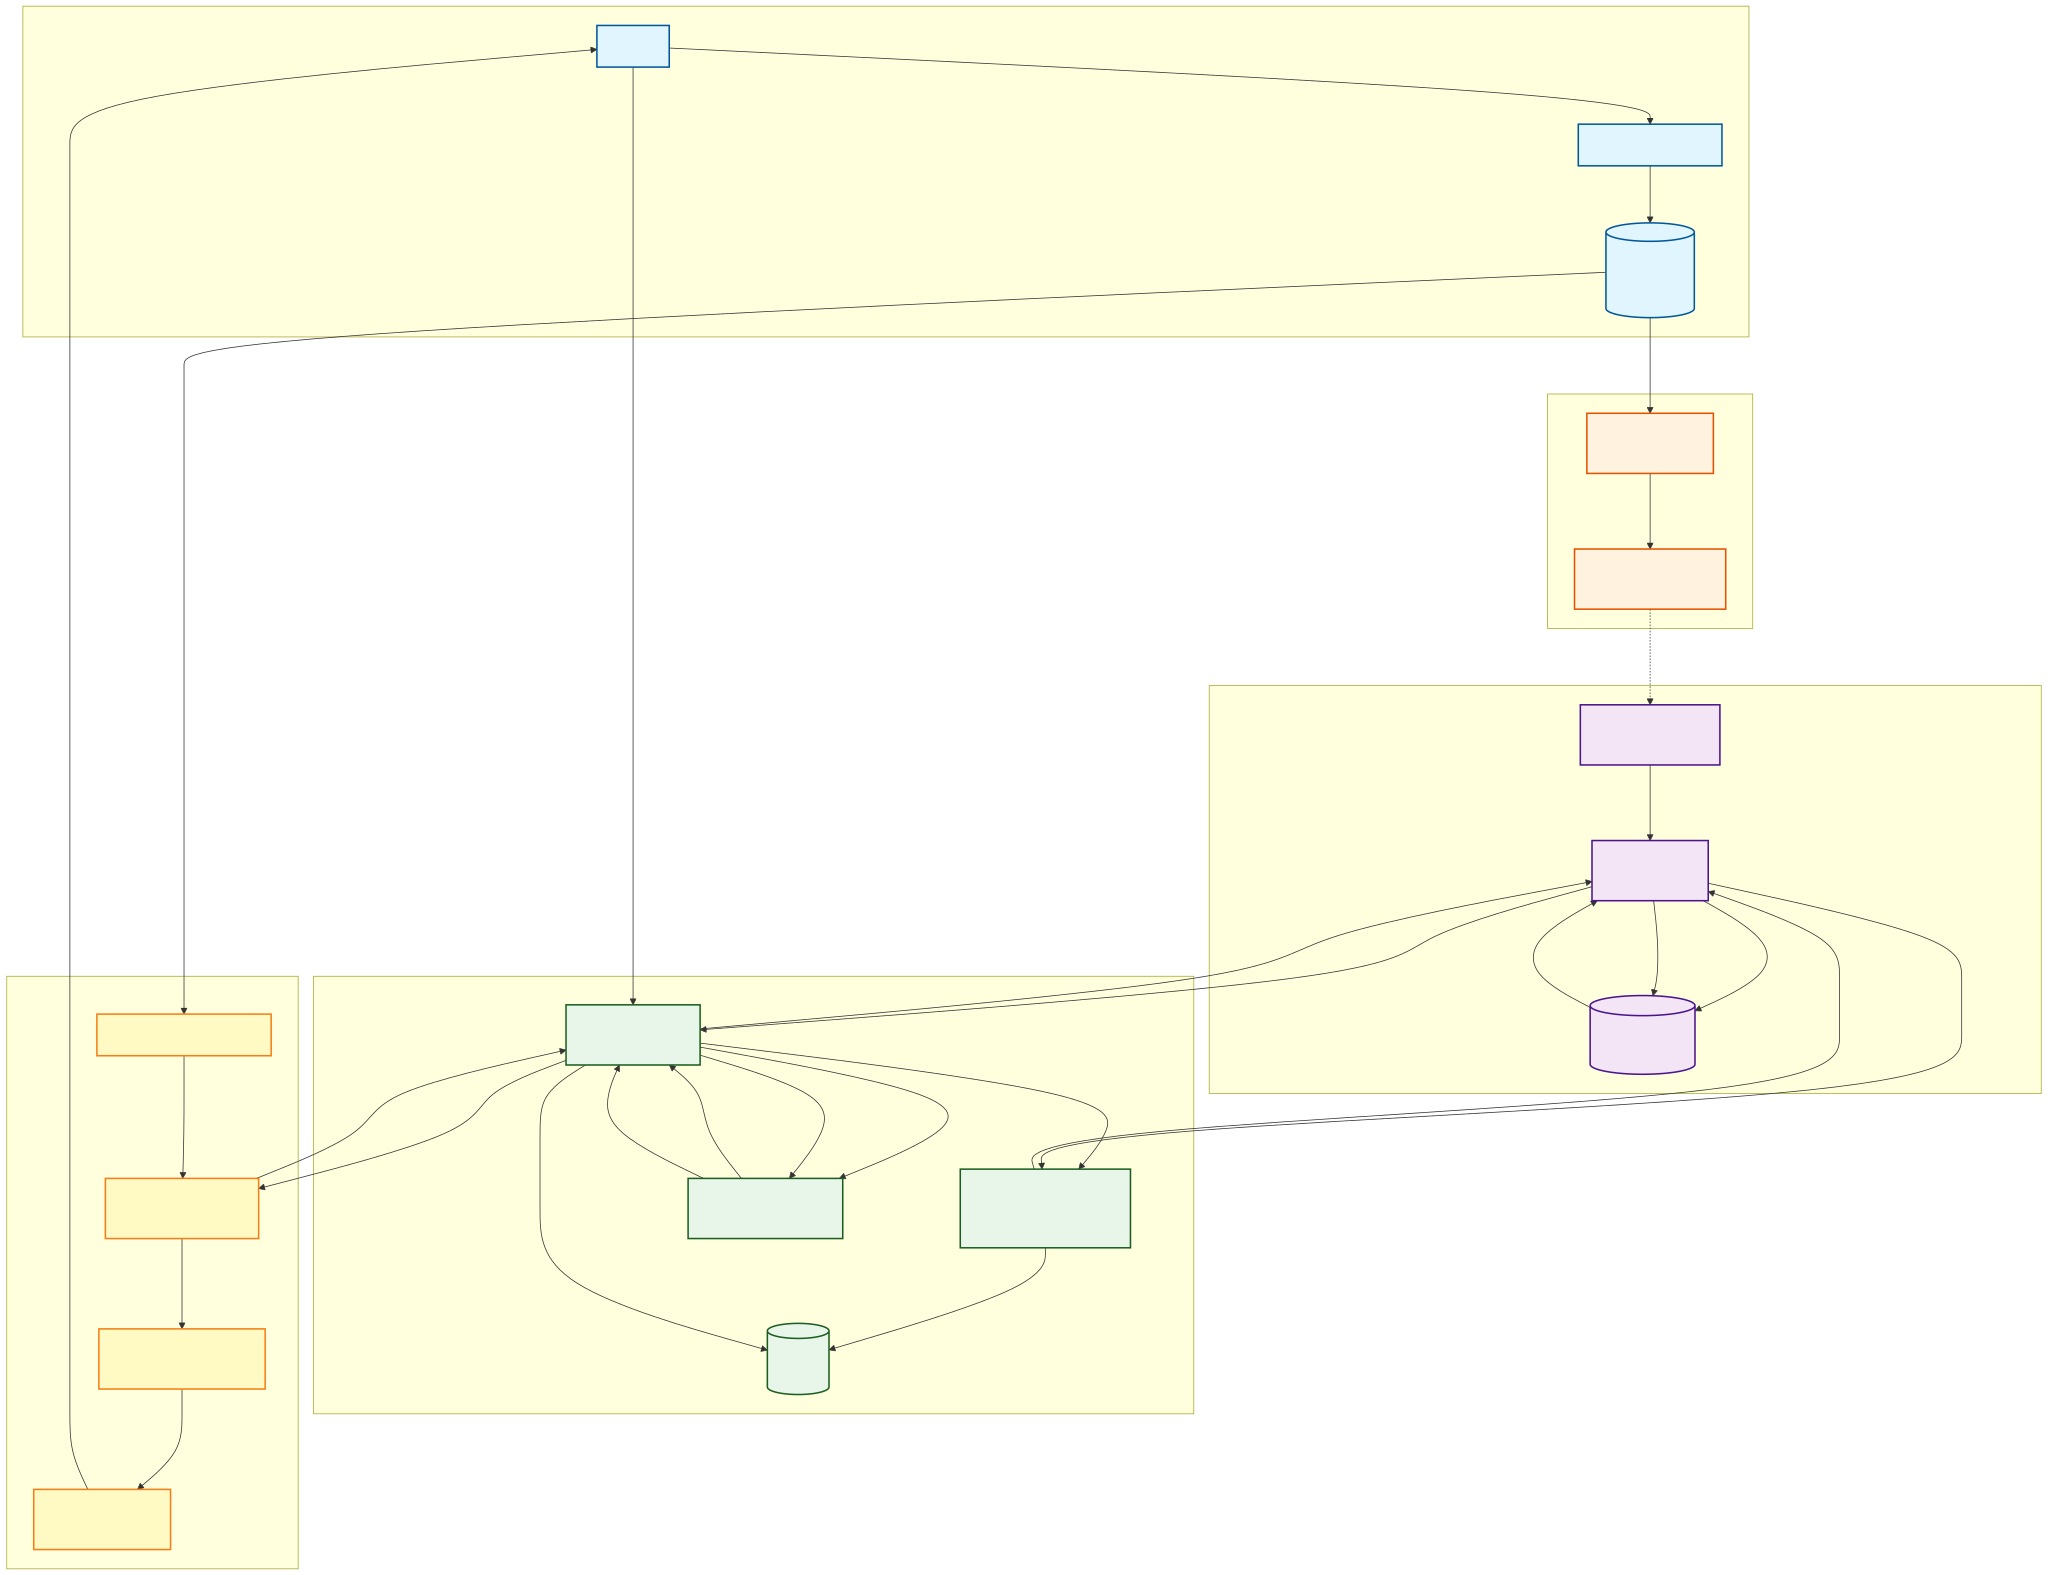
\includegraphics{figures/dataflow_diagram.png}}
    \caption{Macless-Haystack Architecture and Data Flow}
    \label{fig:architecture}
\end{figure}

\subsection{LINDDUN Privacy Threat Analysis}
The following table (Table~\ref{tab:lindunn}) presents a systematic analysis of privacy threats using the LINDDUN framework, which categorizes threats across privacy dimensions: Linkability, Identifiability, Non-repudiation, Detectability, Disclosure of information, Unawareness, and Non-compliance. Many compliance-related threats stem from the project's reverse-engineering of Apple's proprietary protocol and operation outside Apple's official ecosystem, which cannot be fully resolved without changing the project's purpose.

\begin{longtable}{|>{\raggedright\arraybackslash}p{1.1cm}|>{\raggedright\arraybackslash}p{2cm}|>{\raggedright\arraybackslash}p{3.2cm}|>{\raggedright\arraybackslash}p{1.8cm}|>{\raggedright\arraybackslash}p{1.1cm}|>{\raggedright\arraybackslash}p{3.2cm}|}
\caption{LINDDUN Privacy Threat Analysis}\label{tab:lindunn}\\
\hline
\textbf{Code} & \textbf{Threat Category} & \textbf{Description} & \textbf{Affected Interaction(s)} & \textbf{Severity} & \textbf{Mitigation} \\
\hline
\endfirsthead
\hline
\textbf{Code} & \textbf{Threat Category} & \textbf{Description} & \textbf{Affected Interaction(s)} & \textbf{Severity} & \textbf{Mitigation} \\
\hline
\endhead
\hline
\endfoot
NC.3 / II.1 & Non-Compliance & Apple ID and password can be stored in plain text in config.ini (optional but supported). Exposes credentials to anyone with filesystem access (to the Macless-Haystack server). Similar for auth.json & Interaction 8, 14, 13 & Critical & Remove plain text password storage; require interactive login only \\
\hline
DD.4.2 / NC.2 & Data Disclosure / Non-Compliance & Storage of private and public keys in plain text. Keys should be stored using platform-specific secure storage (Apple Keychain, Android Keystore, GNOME Keyring, Windows Credential Manager). & Interaction 2, 3b & High & Implement secure key storage using platform APIs (e.g., flutter\_secure\_storage) \\
\hline
L.1.1 / I.2.2.b & Linkability / Information Disclosure & Static advertisement keys allow tracking of device presence. The system broadcasts the same public key continuously, enabling anyone to determine if the tracked device (and by extension, its owner) is nearby. & Interaction 4 & High & Implement key rotation mechanism (firmware currently rotates every 30 min for multi-key setups) \\
\hline
NC.3.c & Non-Compliance & Weak authentication: no authentication required by default, or single username/password shared among all users of an endpoint instance. & Interaction 15, 16, 17, 24 & High & Implement per-user authentication; support OAuth or token-based auth \\
\hline
U.1.2 & Unawareness & Users are not informed that sharing their private key with others enables complete location tracking of their device. Lacks clear privacy warnings. & Interaction 2 & Medium & Add explicit privacy warnings in documentation and UI when exporting keys \\
\hline
NC.1.2.a & Regulatory Non-Compliance & Violation of Apple's EULA by creating custom AirTag-like devices using Apple's Find My network infrastructure. & Interaction 3a, 4 & Medium & Add legal disclaimer; users assume responsibility \\
\hline
D.3 & Detectability & Static advertisement keys allow querying Apple servers to determine if a tracker is still active by checking for new location reports, even without decryption. & Interaction 4, 20 & Medium & Key rotation partially mitigates this; inherent to Find My protocol \\
\hline
NR.1.1.a & Non-Repudiation & Apple ID is attached to all location report requests, allowing Apple to identify and track Macless-Haystack server hosters and their query patterns. & Interaction 8, 11, 12, 13, 20 & Medium & Inherent to Apple's authentication; no mitigation without protocol changes \\
\hline
NC.1.2.b & Regulatory Non-Compliance & Reverse engineering and accessing iCloud authentication from non-Apple devices violates Apple's EULA & Interaction 11, 12, 13 & Medium & Legal disclaimer; users assume legal responsibility \\
\hline
L.2.2.1 & Linkability & Sending advertisement keys to potentially public endpoint links user's IP address with their tracked devices. & Interaction 15, 16 & Medium & Only use trusted, self-hosted endpoints; implement end-to-end encryption for API \\
\hline
NC.3.b & Non-Compliance & HTTP access is supported (non-mandatory HTTPS), exposing advertisement keys during transmission. Man-in-the-middle attackers can capture key. & Interaction 15, 16, 24 & Medium & Enforce HTTPS mandatory; disable HTTP in production \\
\hline
I.1.2 & Information Disclosure & Apple servers receive query metadata (timestamps, query frequency, advertisement key hashes) revealing usage patterns. & Interaction 20, 21 & Medium & Inherent to protocol; rate limiting and query batching can reduce exposure \\
\hline
\end{longtable}

\subsection{GDPR Compliance Considerations}
To assess GDPR compliance, we analyze the system based on the data controllers involved, the personal data they process, and the specific regulatory risks they face.

\subsubsection{Data Controllers, Personal Data, and Risks}

\paragraph{The End User}
The individual user acts as a data controller because they generate the private keys and define the purpose of the tracking (i.e., deciding which objects or individuals to track).

\textbf{Personal Data Processed:} Private keys, definitions of tracked objects.

\textbf{GDPR Risks:}

\textbf{Household Exemption:} Generally, for purely personal or household activities, the GDPR may not apply under the \textit{household exemption} (Article 2(2)(c)). However, if the user tracks individuals outside of a household context, they become fully liable.

\textbf{Integrity and Confidentiality (Article 5 and Article 32):} The generation of private keys is currently insecure. Before flashing, keys are stored in plaintext JSON and must be imported into the application, preventing the use of secure platform storage (e.g., Keychain, Gnome Keyring).

\textbf{Lawfulness of Processing (Article 6):} The system circumvents Apple's built-in anti-stalking protections. This allows users to track individuals or objects without consent more easily than within the official ecosystem, raising significant ethical and legal concerns regarding non-consensual surveillance.

\paragraph{The Macless-Haystack Endpoint Operator}
The operator of the Macless-Haystack instance acts as the primary data controller for the deployment. They hold the most personal data.

\textbf{Personal Data Processed:}

\emph{Account Credentials:} Apple ID and Password, and derived tokens (DSID, SearchPartyToken, etc.).

\emph{Target Search Data:} Search Keys (IDs) for specific devices.

\emph{Location Data:} Encrypted location reports, decoded metadata, and raw payloads.

\emph{Logged Data:} Debug logs potentially persisting sensitive information.

\textbf{GDPR Risks \& Violations:}

\textbf{Integrity and Confidentiality:} There are critical failures regarding security. Apple ID credentials can be stored in plaintext (e.g., in \texttt{auth.json}), and the frontend supports unencrypted HTTP communication. This exposes potentially personal data to unauthorized access. (it becomes personal data if the middleman is able to link the data to a specific person, eg has the private key or is able to physically track the device using its static key advertisements)

\textbf{Transparency and Purpose Limitation:} A major deficiency is the lack of transparency. The end user (if different from the operator) is often not informed about the processing of their data, and there is no documented purpose specification. If static keys are used, the end user should also be informed that apple might process personal data, depending on if apple can link the static keys to a specific person.

\paragraph{Apple}
Apple processes the encrypted location reports and public advertisement keys uploaded by finder devices.

\textbf{Personal Data Processed:} Encrypted location reports, advertisement keys, uploader IP addresses/Apple IDs.

\textbf{GDPR Risks:}

\textbf{Linkability:} In a self-hosted setup where the tracker owner is the endpoint operator, Apple could link the tracker to the owner's Apple ID, making the data personal.

\textbf{Mitigation:} If rolling keys are used, Apple's ability to link reports to a single device is significantly reduced, arguing for a lack of personal data processing in that specific context.

\subsubsection{Disclaimer on Research Usage}
It is important to note that this application is intended as a proof-of-concept research project. The project repository includes a disclaimer stating: "I take NO responsibility and/or liability for how you choose to use any of the source code available here. By using any of the files available in this repository, you understand that you are AGREEING TO USE AT YOUR OWN RISK. Once again, ALL files available here are for EDUCATION and/or RESEARCH purposes ONLY." 
Consequently, operators hosting an endpoint should be aware of these risks and limit usage to personal research or household activities, avoiding deployment as a general-purpose service.
\subsection{Main Identified Privacy Threats}

\subsubsection{Advertisement Keys in Macless Haystack}
In the current setup, each tracker continuously broadcasts a beacon containing the same static public key so that nearby Apple devices can hear it and create encrypted location reports. Any Apple device that receives such a beacon, takes its own location and encrypts that location to send it to Apple's servers, where only the trackers matching private key can decrypt it. Using a static public key introduces a serious linkability privacy problem. Because the same identifier is broadcasted in every packet, any nearby device with a simple BLE sniffer can record this constant over time and across different places, and then correlate all sightings as belonging to the same physical tracker. This means that anyone could build a detailed movement profile of the tagged object or person just by re-observing the same static key at different locations, even though they cannot decrypt the underlying Find My location reports. The root cause of the privacy threat is therefore not that the encryption is weak, it is that the identifier used as input to the encrypted reporting process is long-lived and public. The encryption protects the content of each report from being read, but it does nothing to stop third parties from recognizing that "this is the same beacon as yesterday" and inferring sensitive patterns (home, workplace, daily routines) purely from repeated radio observations tied to an unchanging public key.
\\
\begin{itemize}
    \item \textbf{unit test:} A dedicated testing environment and test suite were developed to evaluate and validate privacy-related behaviors in the tracker firmware, which had not previously undergone testing. To determine if static keys are being utilized, the \texttt{run\_openhaystack} function is called repeatedly while a shim replaces the Bluetooth advertising routine, enabling direct inspection of the broadcast payloads. Static codes are detected if multiple calls to \texttt{run\_openhaystack} trigger the BLE controller with identical payloads.\footnote{The firmware supports the use of multiple static keys; however, it was tested in a configuration where only a single key was loaded.}
\end{itemize}
\subsubsection{Plain Text Credentials}
The user's Apple ID credentials are stored in plaintext on the Macless-Haystack server inside the auth.json file. This means that anyone with file access to the server can read the user's credentials. This represents a serious security vulnerability that must be addressed immediately, especially when the server and client are managed by different individuals. Additionally, the frontend website is not protected by HTTPS, and communication between the frontend and the Macless-Haystack server is transmitted without encryption. This creates a severe security risk if a user enters their credentials for the Macless-Haystack server into the frontend, as the information would be sent over the network unencrypted. While the current implementation does not require users to enter their credentials, since they are provided during server setup, an uninformed user might still attempt to do so. In scenarios where the server is configured by a third party, entering credentials through the website may even be necessary for the system to function, further increasing the risk.

\todo[inline]{Add unit test for plain text credentials}


% Part 3: Recommendations (no specific word limit mentioned, but part of 4000 word total)
\section{Recommendations}
\subsection{Handeling the GDPR and EULA violations}



\subsection{Mitigating Linkability with Rolling Codes}
Static advertisement keys allow anyone to track a device by listening for its constant signal. To fix this, we recommend using rolling codes, which means the key changes periodically (for example, every 15 minutes). This prevents strangers from linking different signals to the same device, but the owner can still find it because they have the secret key to calculate the list of all past and future IDs.\\
To prevent this we can use the same method as Apple's official airtags \cite{DBLP:journals/corr/abs-2103-02282}. This uses Elliptic Curve Cryptography on the NIST P-224 curve. It starts with a master key pair and a 32-bit symmetric key. New keys are created using the ANSI X.963 key derivation function (KDF) with these formulas:
\begin{align}
SK_i &= \text{KDF}(SK_{i-1}, \text{``update''}, 32) \\
(u_i, v_i) &= \text{KDF}(SK_i, \text{``diversify''}, 72) \\
d_i &= (d_0 * u_i) + v_i \\
p_i &= d_i * G
\end{align}

This requires a small firmware update. The following code snippet shows the main rolling key logic implemented on the tracker:

\begin{lstlisting}[style=cstyle, language=C, caption={Rolling Key Implementation}]
/**
 * @brief Main rolling key logic
 * 1. Rotate Symmetric Key
 * 2. Generate u, v scalars
 * 3. Calculate new Private Key
 * 4. Derive new Public Key
 */
void roll_key_and_update_state() {
    uint8_t next_sym_key[32];
    uint8_t diversify_material[72];
    uint8_t u_bytes[36];
    uint8_t v_bytes[36];
    uint8_t rolling_priv_bytes[28];
    ESP_LOGI(LOG_TAG, "Rolling keys...");

    // 1. Update Symmetric Key: SK_new = KDF(SK_old, "update", 32)
    ansi_x963_kdf(current_symmetric_key, 32, "update", 32, next_sym_key);

    // global state update
    memcpy(current_symmetric_key, next_sym_key, 32);

    // 2. Derive u, v: KDF(SK_new, "diversify", 72)
    ansi_x963_kdf(next_sym_key, 32, "diversify", 72, diversify_material);
    memcpy(u_bytes, diversify_material, 36);
    memcpy(v_bytes, diversify_material + 36, 36);

    // 3. Math: d_i = (d_0 * u + v) mod n
    mbedtls_mpi d_0, u, v, n, d_i, temp;
    mbedtls_mpi_init(&d_0); mbedtls_mpi_init(&u); mbedtls_mpi_init(&v);
    mbedtls_mpi_init(&n);   mbedtls_mpi_init(&d_i); mbedtls_mpi_init(&temp);

    mbedtls_mpi_read_string(&n, 16, P224_ORDER_HEX);

    mbedtls_mpi_read_binary(&d_0, master_private_key, 28);
    mbedtls_mpi_read_binary(&u, u_bytes, 36);
    mbedtls_mpi_read_binary(&v, v_bytes, 36);

    // temp = d_0 * u
    mbedtls_mpi_mul_mpi(&temp, &d_0, &u);
    // d_i = temp + v
    mbedtls_mpi_add_mpi(&d_i, &temp, &v);
    // d_i = d_i mod n
    mbedtls_mpi_mod_mpi(&d_i, &d_i, &n);

    // Export result
    mbedtls_mpi_write_binary(&d_i, rolling_priv_bytes, 28);
    ESP_LOGI(LOG_TAG, "New Private Key:");
    {
        char key_str[28 * 2 + 1];
        for (int i = 0; i < 28; i++) {
            sprintf(&key_str[i * 2], "%02x", rolling_priv_bytes[i]);
        }
        key_str[28 * 2] = '\0';
        ESP_LOGI(LOG_TAG, "%s", key_str);
    }

    // Cleanup MPI
    mbedtls_mpi_free(&d_0); mbedtls_mpi_free(&u); mbedtls_mpi_free(&v);
    mbedtls_mpi_free(&n);   mbedtls_mpi_free(&d_i); mbedtls_mpi_free(&temp);

    // 4. Derive Public Key
    derive_public_key_bytes(rolling_priv_bytes, 28, current_public_key);
}
\end{lstlisting}

The tracker needs to store the master keys and a function to calculate the new ones. The tracker needs to store the master keys and a function to calculate the new ones. This is easy to do on chips like the ESP32 or nrf5x. We tested this approach and confirmed its functionality. Additionally, the tracker should also save the current key to memory so it doesn't lose its place if the battery dies.
The major downside of this approach is that if the key-rolling interval is set to a short value, the tracker can evade Apple’s built-in anti-stalking features. As a result, unlike regular AirTags, people may not receive alerts when an unknown tracker is following them allowing \cite{10.1145/3463676.3485616}.
\subsubsection{Client-Side Challenges}
Updating the user application is challenging because custom trackers are less reliable than official AirTags, and users may not open the application for weeks or even months at a time.

As a result, when a user returns to the application after a long period of inactivity, we cannot assume that the current AirTag code is simply the last known code incremented by the elapsed time. The tracker may have been powered off for a significant portion of that period, making the actual code state unpredictable.

This uncertainty forces us to search backward from the estimated current code to the last known code. However, performing this search naively risks triggering Apple server rate limits or bans. Additionally, there is currently no built-in mechanism to resynchronize the tracker with the application.

Resynchronization could be implemented through Bluetooth or NFC, or by integrating an RTC module into the tracker. An RTC would provide accurate timekeeping, allowing the application to reliably calculate code updates even after extended powered off periods\footnote{RTC modules typically include a built-in backup battery to maintain timekeeping when the host device is unpowered. Battery life can range from several months to over ten years, depending on usage. In our use case, the RTC would only draw backup power when the tracker is turned off, resulting in a multi-year battery lifespan.}

\section{Conclusion}
\todo[inline]{Add conclusion summarizing key findings and recommendations}

\bibliographystyle{plain}
\bibliography{references}


\end{document}